% ---
\chapter{Algoritmos de compressão sem perda}
% ---

Com no que foi apresentado no capítulo anterior, a compressão de dados pode ser vista como uma sub-área da teoria da informação. O principal objeto de estudo é o desenvolvimento métodos e ferramental (ou otimização dos já existentes) que reduzam a quantidade de dados necessários para representar uma determinada informação.

Os algoritmos de compressão podem ser categorizadas em duas diferentes classes: os de compressão \textbf{com perda} e \textbf{sem perda}. Os \textbf{algoritmos de compressão sem perda} admitem uma baixa porcentagem de perda de informações durante a codificação para obter maior performance, muito uteis na transmissão de dados em streaming por exemplo. Nos \textbf{algoritmos de compressão com perda} o processo de codificação deve ser capaz de recuperar os dados em sua totalidade, geralmente utilizados em casos onde não pode haver perda de informações (como por exemplo, compressão de arquivos de texto).

\pagebreak

\section{Código de Huffman} \label{sec:huff}
O \textbf{algoritmo de Huffman} (desenvolvido por David Huffman em 1952) é um dos componentes mais utilizados em algoritmos de compressão sem perda, servindo como base para algoritmos como o Deflate (utilizado amplamente na web).
Os códigos gerados a partir do algoritmos de Huffman são chamados \textbf{Códigos de Huffman}.

O código de Huffman é descrito em termos de como ele gera uma árvore de código livre de prefixo. Considere o conjunto de mensagens \emph{M}, com $p_i$ sendo a probabilidade associada a $m_i$

\begin{algorithm}[H]
\caption{Algoritmo de Huffman} \label{alg:huff}
\begin{algorithmic}
	\State $Forest \gets \emph{[]}$\\
	\ForAll{$m_i \in M$} \Comment{Inicializando floresta}
		\State $T \gets newTree()$
		\State $node \gets newNode()$
		\State $node.weight \gets p_i$ \Comment{$w_i = p_i$}
		\State $T.root \gets node$
		\State $Forest.append(T)$ \Comment{Adiciona um nova arvore na floresta}
	\EndFor \\
	
	\While{$Forest.size > 1$}
		\State $T1 \gets ExtractMin(Forest)$ \Comment{Retorna a árvore cuja raiz é mínima, e retira da floresta}
		\State $T2 \gets ExtractMin(Forest)$
		\State $HTree \gets newTree()$
		\State $HTree.root \gets newNode()$ \\
		\State $HTree.root.left \gets T1.root$
		\State $HTree.root.right \gets T2.root$
		\State $HTree.root.weight \gets T1.root.weight + T2.root.weight$
		\State Forest.append(HTree) 
	\EndWhile
\end{algorithmic}
\end{algorithm}

\subsection{Análise assintótica}
Seja \emph{n} o tamanho do conjunto de mensagens \emph{M}. Para que o algoritmo percorra toda a floresta, formada por uma árvore para cada $\emph{m} \in \emph{M}$, serão necessárias \emph{n} interações.
Considerando que as funções \emph{ExtractMin()} e \emph{.append()} foram construídas a partir de uma fila de prioridades de \textbf{heap}, o algoritmo será executado em  $O(n \log_2 n)$.

\subsection{Corretude}
O teorema a seguir (escrito por Huffman) mostra a principal propriedade do Algoritmo de Huffman, os códigos de Huffman são códigos ótimos e livres de prefixo.


\begin{lemma} \label{lemma:dist_prob_avg_size} Seja \emph{C} um código ótimo livre de prefixo, com $\{ p_1, p_2,..., p_n\}$ sendo a distribuição de probabilidades associada ao código. Se $p_i > p_j$ então $l(w_i) \leq l(w_j)$

\begin{proof} 
Assuma que $l(c_i) > l(c_j)$. Agora vamos construi um novo código \emph{C'}, trocando $w_i$ por $w_j$. Dado $l_a$ como o comprimento médio do código \emph{C}, o código \emph{C'} terá o seguinte comprimento:
\begin{align*}
l'_a &= l_a + p_j(l(w_i) - l(w_j)) + p_i(l(w_j) - l(w_i)) \\
&= l_a + (p_j - p_i)(l(w_i) - l(w_j)) 
\end{align*}

Pelas suposições feitas anteriormente o termo $(p_j - p_i)(l(w_i) - l(w_j))$ seria negativo, contradizendo o fato do código \emph{C} ser um código ótimo e livre de prefixo (pois neste caso $l'_a > l_a$).

\textbf{Nota*} : Perceba que em uma árvore de Huffman, o tamanho da palavra código $w_i$ também representa seu nível na árvore.
\end{proof}
\end{lemma}

\begin{theorem} O algoritmo de Huffman gera um código ótimo livre de prefixo.
\begin{proof}
A prova se dará por indução sobre o número de mensagens pertencentes ao código. Vamos mostrar que se o Algoritmo de Huffman gera um código livre de prefixo ótimo para qualquer distribuição de probabilidades com \emph{n} mensagens, então o mesmo ocorre para \emph{n + 1} mensagens.

\item \textbf{Caso Base.} Para n = 2 o teorema é trivialmente satisfeito considerando um código que atribui um bit pra cada mensagem do código.

\item \textbf{Passo indutivo}. Pelo lema \ref{lemma:dist_prob_avg_size} sabemos que as menores probabilidades estão nos menores níveis da árvore de Huffman (por ser uma árvore completa binário, o seu menor nível deve possuir ao menos dois nós). Já que esses nós possuiriam o mesmo tamanho, podemos muda-los de posição sem afetar o tamanho médio do código, concluindo assim que estes são nós \textbf{irmãos}.\\
Agora defina um conjunto de mensagens \emph{M} de tamanho \emph{n + 1} onde T é a árvore de prefixo ótima construída a partir do Algoritmo de Huffman aplicado em \emph{M}. Vamos chamar os dois nós de menor probabilidade na árvore de \emph{x} e \emph{y} (que pelo argumento anterior, são nós irmãos). Vamos construir uma nova árvore \emph{T'} a partir de \emph{T} removendo os nós \emph{x} e \emph{y}, fazendo assim que o pai destes nós, que chamaremos de \emph{z}, seja o de menor probabilidade (de acordo com a definição do Algoritmo de Huffman, $p_z = p_y + p_x$). Considere \emph{k} como a profundidade de \emph{z}, temos:

\begin{align*}
l_a(T) &= l_a(T') + p_x(k + 1) + py(k + 1) - p_z k \\
&= l_a(T') + p_x + p_y
\end{align*}

Sabemos pela hipótese de indução que $l_a(T')$ é mínimo, pois \emph{T'} tem o tamanho \emph{n} e foi gerada pelo algoritmo de Huffman. Note que independente da ordem que forem inseridos, os nós \emph{x} e \emph{y} irão adicionar a constante $p_z = p_x + p_y$ no peso médio do código. Como $l_a(T')$ é mínimo para um conjunto de mensagens de tamanho \emph{n} e seu nó de menor peso tem distribuição de probabilidade $p_z$, $l_a(T)$ também é mínimo para o conjunto de mensagens \emph{M} e logo \emph{T} é ótimo e livre de prefixo. 
\end{proof}
\end{theorem}

\section{Lempel-Ziv 77 (LZ77)}

\subsection{Algoritmos de Lempel-Ziv}
Nos anos de 1977 e 1978, Jacob Ziv e Abraham Lempel publicaram dois artigos apresentando os algoritmos (\textbf{LZ77} e \textbf{LZ88}) que futuramente serviriam como base para toda uma família de algoritmos de compressão (conforme mostrado na Figura~\ref{fig:lz77}), chamados de algoritmos de Lempel-Ziv.
Os algoritmos de Lempel-Ziv realizam o processo de compressão baseado em um \textbf{dicionário} de símbolos vistos anteriormente (diferente do \nameref{alg:huff}, que utiliza a probabilidade associada a cada símbolo). 
Ambos tem um funcionamento parecido, que se resume em substituir partes da entrada por referências à partes iguais anteriormente processadas, e diferem na maneira em que procuram por repetições a serem substiruídas. 

\begin{figure}[h]
   \centering
   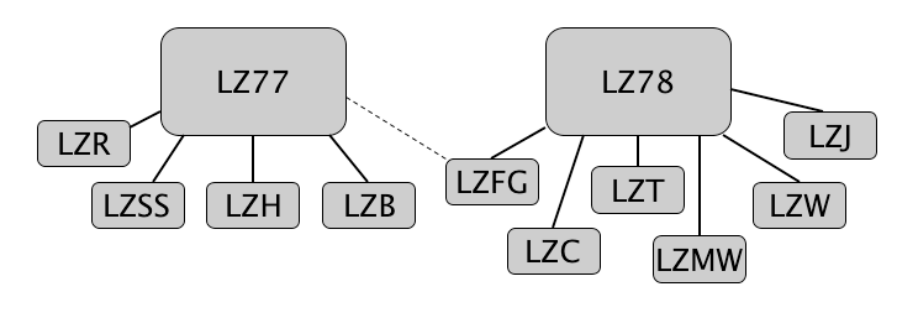
\includegraphics[scale=0.75]{figs/lz77fam.png}
    \caption{Familia de algoritmos Lempel Ziv}
    \label{fig:lz77}
 \end{figure}

\subsection{Descrição do LZ77}
O LZ77 e suas variações utilizam a técnica de \emph{janela deslizante} para encontrar cadeias de símbolos correspondentes. A janela é dividida em duas partes separadas por um \emph{cursor} (que se move conforme novos símbolos são codificados).

Os elementos à esquerda do cursor são chamados \emph{dictionary} e contém todos os elementos codificados, já os elementos à direita do \emph{cursor} são chamados de \emph{lookahead buffer}.
A ideia geral do algoritmo é substituir os símbolos do \emph{lookahead buffer} por \emph{tokens}, onde cada \emph{token} é constituído por uma tupla que ``aponta'' para a maior cadeia de elementos no \emph{dictionary} que correspondem aos elementos que estão no início do \emph{lookahead buffer}.

\begin{algorithm}[H]
\caption{Algoritmo Lempel-Ziv 77} \label{alg:lz77}
\begin{algorithmic}

	\State $cursor \gets 0$
	\State $tokens \gets []$

	\While{$cursor < M.size()$}
		\State $position, len \gets findBestMatch(M, cursor)$
		\If{$len > 0$}
			$tokens.append([position, len, null])$
			\State $cursor \gets cursor + len$
		\Else
			$tokens.append((0, 0, M[cursor]))$
			\State $cursor \gets cursor + 1$
		\EndIf
	\EndWhile
\end{algorithmic}
\end{algorithm}




